%!TEX root = ./template-skripsi.tex
%-------------------------------------------------------------------------------
%                            BAB III
%               			PEMBAHASAN
%-------------------------------------------------------------------------------

\chapter{METODOLOGI PENELITIAN}

\section{Tahapan Penelitian}

Terdapat tahapan-tahapan yang harus dilalui untuk melaksanakan penelitian ini. Tahapan penelitian dapat dilihat pada diagram \ref{gambar:tahapan_penelitian}. Terdapat beberapa algoritma yang belum dijelaskan sebelumnya seperti Modified DPC (MDPC) dan Random Walker. Algoritma MDPC dirumuskan karena kekurangan dari algoritma DPC yang akan dijelaskan pada bagian selanjutnya. Sedangkan algoritma Random Walker merupakan program yang mensimulasikan pergerakan kunjungan halaman web dan merupakan basis dari algoritma Pagerank \citep{ilprints422}, sehingga sangat cocok untuk dijadikan sebagai acuan untuk melakukan verifikasi hasil.

\begin{figure}[H]
	\centering
	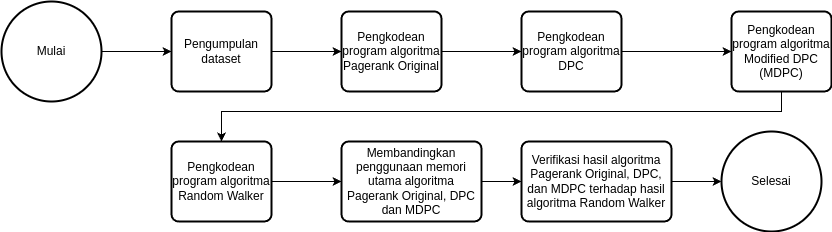
\includegraphics[keepaspectratio, width=\textwidth]{gambar/tahapan_penelitian.png}
	\caption{Diagram tahapan penelitian}
	\label{gambar:tahapan_penelitian}
\end{figure}

\section{Pengumpulan Dataset}

Penelitian ini menggunakan data yang berasal dari basis data penelitian \citet{khatulistiwa2022SearchEngine} ditambah dengan mengumpulkan data tambahan yang sama-sama diperoleh dengan menjalankan program \textit{crawling}. Data yang diperoleh disimpan ke dalam basis data MySQL dan terdapat 13 tabel atau \textit{entity} yang strukturnya dapat dilihat pada tabel-tabel berikut:
	
\begin{table}[h!]
	\centering
	\caption{Struktur tabel \textit{crawling}}
	\label{table:entity_crawling}
	\begin{tabular}{|c|c|c|}
		\hline
		\multicolumn{3}{|c|}{\textit{crawling}} \\
		\hline
		\textbf{No.} & \textbf{Atribut} & \textbf{Tipe Data} \\
		\hline
		1. & id\_crawling & int \\
		2. & start\_urls & text \\
		3. & keyword & text \\
		4. & total\_page & int \\
		5. & duration\_crawl & time \\
		6. & created\_at & timestamp \\
		\hline
	\end{tabular}
\end{table}
 
 \begin{table}[h!]
	\centering
	\caption{Struktur tabel \textit{page\_information}}
	\label{table:entity_page_information}
	\begin{tabular}{|c|c|c|}
		\hline
		\multicolumn{3}{|c|}{\textit{page\_information}} \\
		\hline
		\textbf{No.} & \textbf{Atribut} & \textbf{Tipe Data} \\
		\hline
		1. & id\_page & int \\
		2. & crawl\_id & int \\
		3. & url & text \\
		4. & html5 & tinyint \\
		5. & title & text \\
		6. & description & text \\
		7. & keywords & text \\
		8. & content\_text & text \\
		9. & hot\_url & tinyint \\
		10. & size\_bytes & bigint \\
		11. & model\_crawl & text \\
		12. & duration\_crawl & time \\
		13. & created\_at & timestamp \\
		\hline
	\end{tabular}
\end{table}

\begin{table}[h!]
	\centering
	\caption{Struktur tabel \textit{tfidf\_word}}
	\label{table:tfidf_word}
	\begin{tabular}{|c|c|c|}
		\hline
		\multicolumn{3}{|c|}{\textit{tfidf\_word}} \\
		\hline
		\textbf{No.} & \textbf{Atribut} & \textbf{Tipe Data} \\
		\hline
		1. & id\_word & int \\
		2. & word & text \\
		3. & page\_id & int \\
		4. & tfidf\_score & double \\
		\hline
	\end{tabular}
\end{table}

\begin{table}[h!]
	\centering
	\caption{Struktur tabel \textit{tfidf}}
	\label{table:entity_tfidf}
	\begin{tabular}{|c|c|c|}
		\hline
		\multicolumn{3}{|c|}{\textit{tfidf}} \\
		\hline
		\textbf{No.} & \textbf{Atribut} & \textbf{Tipe Data} \\
		\hline
		1. & id\_tfidf & int \\
		2. & keyword & text \\
		3. & page\_id & int \\
		4. & tfidf\_total & double \\
		\hline
	\end{tabular}
\end{table}

\begin{table}[h!]
	\centering
	\caption{Struktur tabel \textit{pagerank}}
	\label{table:entity_pagerank}
	\begin{tabular}{|c|c|c|}
		\hline
		\multicolumn{3}{|c|}{\textit{pagerank}} \\
		\hline
		\textbf{No.} & \textbf{Atribut} & \textbf{Tipe Data} \\
		\hline
		1. & id\_pagerank & int \\
		2. & page\_id & int \\
		3. & pagerank\_score & double \\
		\hline
	\end{tabular}
\end{table}

\begin{table}[h!]
	\centering
	\caption{Struktur tabel \textit{page\_linking}}
	\label{table:entity_page_linking}
	\begin{tabular}{|c|c|c|}
		\hline
		\multicolumn{3}{|c|}{\textit{page\_linking}} \\
		\hline
		\textbf{No.} & \textbf{Atribut} & \textbf{Tipe Data} \\
		\hline
		1. & id\_linking & int \\
		2. & page\_id & int \\
		3. & outgoing\_link & text \\
		\hline
	\end{tabular}
\end{table}

\begin{table}[h!]
	\centering
	\caption{Struktur tabel \textit{page\_tables}}
	\label{table:entity_page_tables}
	\begin{tabular}{|c|c|c|}
		\hline
		\multicolumn{3}{|c|}{\textit{page\_tables}} \\
		\hline
		\textbf{No.} & \textbf{Atribut} & \textbf{Tipe Data} \\
		\hline
		1. & id\_table & int \\
		2. & page\_id & int \\
		3. & table\_str & text \\
		\hline
	\end{tabular}
\end{table}

\begin{table}[h!]
	\centering
	\caption{Struktur tabel \textit{page\_forms}}
	\label{table:entity_page_forms}
	\begin{tabular}{|c|c|c|}
		\hline
		\multicolumn{3}{|c|}{\textit{page\_forms}} \\
		\hline
		\textbf{No.} & \textbf{Atribut} & \textbf{Tipe Data} \\
		\hline
		1. & id\_form & int \\
		2. & page\_id & int \\
		3. & form & text \\
		\hline
	\end{tabular}
\end{table}

\begin{table}[h!]
	\centering
	\caption{Struktur tabel \textit{page\_images}}
	\label{table:entity_page_images}
	\begin{tabular}{|c|c|c|}
		\hline
		\multicolumn{3}{|c|}{\textit{page\_images}} \\
		\hline
		\textbf{No.} & \textbf{Atribut} & \textbf{Tipe Data} \\
		\hline
		1. & id\_image & int \\
		2. & page\_id & int \\
		3. & image & text \\
		\hline
	\end{tabular}
\end{table}

\begin{table}[h!]
	\centering
	\caption{Struktur tabel \textit{page\_scripts}}
	\label{table:entity_page_scripts}
	\begin{tabular}{|c|c|c|}
		\hline
		\multicolumn{3}{|c|}{\textit{page\_scripts}} \\
		\hline
		\textbf{No.} & \textbf{Atribut} & \textbf{Tipe Data} \\
		\hline
		1. & id\_script & int \\
		2. & page\_id & int \\
		3. & script & text \\
		\hline
	\end{tabular}
\end{table}

\begin{table}[h!]
	\centering
	\caption{Struktur tabel \textit{page\_list}}
	\label{table:entity_page_list}
	\begin{tabular}{|c|c|c|}
		\hline
		\multicolumn{3}{|c|}{\textit{page\_list}} \\
		\hline
		\textbf{No.} & \textbf{Atribut} & \textbf{Tipe Data} \\
		\hline
		1. & id\_list & int \\
		2. & page\_id & int \\
		3. & list & text \\
		\hline
	\end{tabular}
\end{table}

\begin{table}[h!]
	\centering
	\caption{Struktur tabel \textit{page\_styles}}
	\label{table:entity_page_styles}
	\begin{tabular}{|c|c|c|}
		\hline
		\multicolumn{3}{|c|}{\textit{page\_styles}} \\
		\hline
		\textbf{No.} & \textbf{Atribut} & \textbf{Tipe Data} \\
		\hline
		1. & id\_style & int \\
		2. & page\_id & int \\
		3. & style & text \\
		\hline
	\end{tabular}
\end{table}

Dari 13 tabel tersebut, nantinya tabel yang akan dipakai adalah tabel \textit{page\_linking}, \textit{page\_information}, dan tabel \textit{pagerank}. Tabel \textit{page\_linking} memuat informasi dari halaman mana \textit{link} berasal melalui atribut \textit{page\_id} dan ke mana \textit{link} tersebut menunjuk melalui atribut \textit{url}. Untuk tabel \textit{page\_information} atribut yang dipakai hanya \textit{id\_page} dan \textit{url}. Lalu setelah perhitungan selesai, maka hasilnya akan disimpan kedalam tabel \textit{pagerank}.

Pada penelitian ini digunakan dua \textit{dataset}. \textit{Dataset} pertama yang nantinya disebut sebagai Dataset 1 merupakan \textit{dataset} gabungan dari \textit{dataset} yang diperoleh dari penelitian \citet{khatulistiwa2022SearchEngine} dan data lanjutan yang diperoleh dengan cara \textit{crawling}. Sebelumnya Dataset 1 hanya memiliki tidak lebih dari 11.000 baris halaman web \textit{page\_information} menjadi 20.493 baris dan 2.915.842 baris \textit{page\_linking}. Data \textit{page\_information} pada Dataset 1 dapat dikelompokan ke dalam 560 \textit{cluster} berdasarkan \textit{domain}-nya yang dapat dilihat pada tabel \ref{domain:dataset1}.

\begin{longtable}{|c|c|c|}
\caption{Data \textit{cluster} pada Dataset 1}
\label{domain:dataset1} \\
\hline
\textbf{No.} & \textbf{Domain} & \textbf{Jumlah Halaman} \\
\hline
1 & detik.com & 2.215 \\
2 & unj.ac.id & 2.208 \\
3 & sport.detik.com & 1.279 \\
4 & finance.detik.com & 1.098 \\
5 & repository.unj.ac.id & 1.089 \\
6 & news.detik.com & 802 \\
7 & oto.detik.com & 779 \\
8 & inet.detik.com & 671 \\
9 & support.google.com & 630 \\
10 & food.detik.com & 626 \\
\vdots & \vdots & \vdots \\
558 & codingcompetitions.withgoogle.com & 1 \\
559 & googledevelopers.blogspot.com & 1 \\
560 & skillshop.exceedlms.com & 1 \\
\hline
\end{longtable}

%filling%
Dapat dilihat pada tabel \ref{domain:dataset1}, halaman web didominasi oleh domain "detik.com" dan "unj.ac.id" beserta sub domainnya, hal ini karena saat dilakukan \textit{crawling} titik halaman web awal-awal yang di-\textit{crawl} adalah "detik.com" dan "unj.ac.id". Hal ini juga membuktikan kecendrungan dari halaman web memiliki \textit{link} yang bersifat \textit{intra-link} yaitu \textit{link} yang menunjuk halaman lain yang masih di dalam satu domain-nya, yang merupakan salah satu basis dari algoritma DPC \citep{zhuetal2005distributedPagerank}. 
%filling end%

Yang kedua, Dataset 2 merupakan \textit{dataset} kecil dan \textit{domain} kecil yang sengaja dikumpulkan untuk melihat perbedaan performa algoritma antara \textit{dataset} yang berisi banyak \textit{domain} besar dengan \textit{dataset} yang berisi \textit{domain} kecil. Batasan pada tiap \textit{domain} yang dipakai ketika mengumpulkan data adalah 20 halaman web per \textit{domain}. Pada Dataset 2 terdapat 100 baris \textit{page\_information}, 5.944 baris \textit{page\_linking}, serta 5 \textit{cluster} atau \textit{domain}. Data \textit{cluster} pada Dataset 2 dapat dilihat pada tabel \ref{domain:dataset2}.

\begin{longtable}{|c|c|c|}
\caption{Data \textit{cluster} pada Dataset 2}
\label{domain:dataset2} \\
\hline
\textbf{No.} & \textbf{Domain} & \textbf{Jumlah Halaman} \\
\hline
1 & unj.ac.id & 20 \\
2 & ppid.unj.ac.id & 20 \\
3 & fip.unj.ac.id & 20 \\
4 & fbs.unj.ac.id & 20 \\
5 & fmipa.unj.ac.id & 20 \\
\hline
\end{longtable}

\section{Kelemahan Algoritma Pagerank Original}

Algoritma Pagerank Original bekerja dengan cara melakukan iterasi perkalian antara vektor \textit{ranking} halaman web terhadap matriks transisi graf situs-situs web. Permasalahan muncul karena matriks transisi tersebut membutuhkan memori utama yang cukup besar, yaitu dengan kompleksitas $O(N^2)$. Misal jika tipe data yang dipakai adalah \textit{floating point} 64 bit dan jika pada dataset terdapat 10 ribu halaman web, maka matriks transisi yang terbentuk adalah matriks persegi 10 ribu $\times$ 10 ribu dan secara memori utama diperlukan $10.000 \times 10.000 \times 64 \text{ bit} = 6.400.000.000 \text{ bit} = 800 \text{ Mega Byte}$. Walaupun pada contoh sebelumnya cukup kecil, pada kenyataannya internet memiliki miliaran halaman web yang, jika menggunakan algoritma Pagerank Original tanpa penanganan khusus, akan memakan \textit{Peta Byte} atau bahkan \textit{Exa Byte} memori. Akibatnya jika dilakukan pada satu mesin komputer pribadi yang hanya menggunakan memori 4 \textit{Giga Byte} sampai 32 \textit{Giga Byte}, program akan \textit{crash}.

\section{Penjelasan Lanjut Algoritma DPC}

Algoritma dimulai dengan memasukan input matriks transisi $P$ dan himpunan \textit{cluster} halaman web $G$. Keduanya didapatkan dari basis data penelitian \citet{khatulistiwa2022SearchEngine}, tersusun atas dua \textit{entity} yang akan dijelaskan pada nanti pada bagian berikutnya. \textit{damping factor} $d$ yang nilainya mengikuti penelitian \citet{zhuetal2005distributedPagerank} yakni $d=0.85$, dan nilai $0 < \epsilon < 1$ untuk toleransi \textit{error}.

Selanjutnya untuk setiap \textit{cluster} $G_i$ dibuat matriks lokal transisi ukuran $N_i \times N_i$ diambil dari nilai matriks transisi $P$. Setelah itu hitung nilai Pagerank lokal $\pi^0_i$ dengan memasukan $Q_i$, nilai toleransi \textit{error} $\epsilon$, dan nilai Pagerank awal-awal adalah $\frac{e}{N_i}$. Ingat $\epsilon = [1,1,...,1]^T$ atau vektor kolom seragam yang semua nilainya satu dan $N_i$ adalah jumlah anggota $G_i$ maka $\frac{e}{N_i}$ = $[\frac{1}{N_i}, \frac{1}{N_i},...,\frac{1}{N_i}]$. Hasil dari Pagerank lokal awal tersebut adalah vektor dengan dimensi $N_i \times 1$.

Langkah selanjutnya sudah memasuki \textit{looping}. $k$ adalah jumlah iterasi. Dibuat matriks agregat $A^k = RPS(\pi^k)$. $R$ adalah matriks $n \times N$, dimana $n$ adalah panjang $G_i$ dan $N$ adalah banyaknya halaman web secara keseluruhan. $R$ didefinisikan pada persamaan \ref{eq:3}. $P$ adalah matriks transisi secara keseluruhan dengan dimensi $N \times N$. $S(\pi^k)$ matriks disagregasi $N \times n$ yang didefinisikan pada persamaan \ref{eq:4}. Matriks $A^k$ dipakai sebagai input matriks transisi untuk perhitungan Pagerank pada level kasar $z^k = Pagerank(A^k, \frac{e}{n}, \epsilon)$. Perlu diingat, karena dimensi $A^k$ adalah $n \times n$, maka dimensi vektor $\frac{e}{n}$ adalah $n \times 1$. Akibatnya dimensi vektor $z^k$ adalah $n \times 1$. Langkah ini disebut dengan solusi kasar \textit{coarse level} \citep{zhuetal2005distributedPagerank}.

Setelah itu, setiap \textit{cluster} $G_i$ buat sebuah matriks $(N_i + 1) \times (N_i + 1)$ lokal transisi yang diperbesar $B^k_i$ seperti persamaan \ref{eq:9}. Pada bagian kiri atas matriks $B^k_i$, $P_{ii}$ adalah matriks transisi lokal \textit{cluster} $G_i$. Pada bagian kiri bawah terdapat perkalian vektor baris $e^T$ dengan dimensi $1 \times N$ dan $P_{*i}$ yang merupakan matriks transisi dari halaman anggota $G_i$ ke halaman anggota $G$ dengan dimensi $N \times N_i$. Hasil akhir dari perkalian tersebut adalah sebuah vektor baris $1 \times N_i$ yang akan menempati baris terbawah dari matriks $B^k_i$ bersama dengan skalar $\alpha^k$, yang menjadi elemen paling bawah dan kanan dari matriks $B^k_i$. Nilai dari $\alpha^k$ tergantung dari jumlah total kolom paling kanan matriks $B^k_i$ yaitu sama dengan 1. Pada bagian kanan atas terdapat matriks $P_{i*}$, berdimensi $N_i \times N$ sekaligus merupakan matriks transisi dari halaman anggota $G$ ke halaman anggota $G_i$, dikalikan dengan matriks disagregasi $S(\pi^k)$ dan vektor $z^k$. Selanjutnya hasil perkalian dari ketiga matriks dan vektor tersebut dikurangi dengan perkalian matriks $P_{ii}$, vektor $\pi^k_i$, dan skalar $z_i$. Dari hasil pengurangan tersebut dibagi dengan pengurangan 1 dikurangi $z^k_i$. Hasil akhir dari operasi bagian kanan atas matriks $B^k_i$ adalah sebuah vektor kolom $N_i \times 1$ sekaligus, bersama $\alpha^k$ merupakan kolom paling kanan dari matriks $B^k_i$.

Selanjutnya hitung algoritma Pagerank dengan masukan matriks $B^k_i$ sebagai matriks transisi, vektor $\frac{e}{(N_i + 1)}$ sebagai vektor \textit{ranking} awal-awal, dan nilai $\epsilon$. Hasil akhir dari Pagerank adalah vektor kolom $N_i \times 1$. Baris pertama sampai baris ke-$N_i$ adalah vektor $\omega^{k+1}_i$ dan baris ke-$(N_i + 1)$ adalah nilai skalar $\beta^{k+1}_i$. Langkah ini disebut sebagai penghalusan (\textit{smoothing}) pada tingkat lebih halus \citep{zhuetal2005distributedPagerank}.

Setelah itu, nilai \textit{ranking} halaman pada tiap \textit{cluster} yang dilambangkan dengan $\pi^{\sim k+1}_i$ diperbaharui dengan melakukan perhitungan sesuai persamaan \ref{alg:3.step:3:3}. Selanjutnya \textit{ranking} halaman tersebut dinormalisasi sesuai persamaan \ref{alg:3.step:normalization}. Hitung selisih \textit{ranking} halaman web iterasi saat ini dengan terasi sebelumnya, jika sudah kurang dari toleransi \textit{error} $\epsilon$ maka algoritma selesai mengembalikan nilai $\pi^{k+1}$. Jika tidak, maka ulangi langkah \textit{looping}.

\section{Kelemahan Algoritma DPC}

Pada algoritma DPC, langkah untuk mendapatkan matriks $A$ memerlukan perkalian matriks $R$, matriks $P$, dan matriks $R(\pi)$. Melakukan perkalian matriks $P$ secara utuh akan menimbulkan masalah dan memakan memori utama yang cukup besar, permasalahan yang sama yang dihadapi pada Pagerank Original. Untuk mengatasi hal tersebut, diperlukan penanganan khusus saat melakukan perkalian agar bisa muat pada memori utama, dengan konsekuensi algoritma dijalankan lebih lambat karena terdapat proses memecah matriks $P$ lebih kecil, dalam penelitian ini memecah matriks $P$ menjadi beberapa vektor kolomnya ketika akan mengalikan matriks $R$ dengan $P$.

Esensi pada langkah empat sampai langkah tujuh algoritma DPC adalah mencari \textit{ranking} domain dan menyesuaikan \textit{ranking} domain tersebut dengan \textit{ranking} halaman web yang masih terisolasi pada domain-nya masing-masing. Matriks $A$ sejatinya adalah matriks transisi domain, sedangkan vektor $z$ adalah vektor \textit{ranking} dari domain. Langkah-langkah tersebut dapat disimplifikasi, pada penelitian ini dirumuskan algoritma modifikasi dari algoritma DPC yang dinamakan algoritma Modified DPC (MDPC).

\section{Algoritma Modified DPC}

Sebelumnya telah dibahas dua algoritma yaitu Pagerank Original pada penelitian \citet{ilprints422}, dan Distributed Pagerank Computation pada penelitian \citet{zhuetal2005distributedPagerank}. Diusulkan algoritma modifikasi dari algoritma DPC atau Modified DPC (MDPC). Secara garis besar MDPC hanya memangkas langkah-langkah pada algoritma DPC, berdasarkan gagasan utama DPC yaitu melakukan perhitungan terpisah \textit{ranking} halaman web berdasarkan \textit{domain}-nya, dan melakukan perhitungan penggabungan dengan menghitung \textit{ranking} \textit{domain} itu sendiri. Masalah utama dari algoritma DPC adalah langkah memperoleh matriks $A$ pada langkah \ref{alg:3.step:2:1} yang melakukan perkalian matriks $P$ secara utuh.

Definisi matriks $A$ versi MDPC yang selanjutnya akan berganti notasi menjadi $A_{mdpc}$ dapat dilihat pada persamaan \ref{eq:a_mdpc}. Makna notasi $P_{**}$ merupakan partisi matriks transisi $P$ yang sudah didefinisikan pada persamaan \ref{eq:6}, sedangkan makna dari \textit{sum} adalah nilai total dari elemen matriks.

\begin{equation}
	\label{eq:a_mdpc}
	A_{mdpc} =
	\begin{pmatrix}
		\frac{\text{sum}(P_{11})}{\text{sum}(P_{*1})} & \cdots & \frac{\text{sum}(P_{1i})}{\text{sum}(P_{*i})} \\
		\vdots & \ddots & \vdots \\
		\frac{\text{sum}(P_{i1})}{\text{sum}(P_{*1})} & \cdots & \frac{\text{sum}(P_{ii})}{\text{sum}(P_{*i})}
	\end{pmatrix}
\end{equation}

Dari web graf di gambar \ref{gambar:web_graph}, dapat dibuat contoh matriks $A_{mdpc}$. Proses perhitungan matriks $A_{mdpc}$ dapat dilihat pada persamaan \ref{eq:a_mdpc_example}.

\begingroup
\makeatletter
\def\f@size{8}
\check@mathfonts
\begin{align*}
	\text{sum}(P_{\ast,1}) = \text{sum}(
		\begin{pmatrix}
			0,02143 & 0,14286 & 0,14286 \\
			0,23393 & 0,14286 & 0,14286 \\
			0,23393 & 0,14286 & 0,14286 \\
			0,23393 & 0,14286 & 0,14286 \\
			0,02143 & 0,14286 & 0,14286 \\
			0,23393 & 0,14286 & 0,14286 \\
			0,02143 & 0,14286 & 0,14286
		\end{pmatrix}
	) = 3,00005 \\
\end{align*}

\begin{align}
	\label{eq:a_mdpc_example}
	\text{sum}(P_{\ast,2}) = \text{sum}(
		\begin{pmatrix}
			0,02143 & 0,14286 \\
			0,02143 & 0,14286 \\
			0,02143 & 0,14286 \\
			0,02143 & 0,14286 \\
			0,44643 & 0,14286 \\
			0,44642 & 0,14286 \\
			0,02143 & 0,14286
		\end{pmatrix}
	) = 2,00002 & &
	\text{sum}(P_{\ast,3}) = \text{sum}(
		\begin{pmatrix}
			0,02143 & 0,14286 \\
			0,02143 & 0,14286 \\
			0,02143 & 0,14286 \\
			0,02143 & 0,14286 \\
			0,02143 & 0,14286 \\
			0,02143 & 0,14286 \\
			0,87143 & 0,14286
		\end{pmatrix}
	) = 2,00003
\end{align}

\begin{align*}
	A_{mdpc} & = &
	\begin{pmatrix}
		\frac{\text{sum}(\begin{pmatrix}
			0,02143 & 0,14286 & 0,14286 \\
			0,23393 & 0,14286 & 0,14286 \\
			0,23393 & 0,14286 & 0,14286
		\end{pmatrix})}{3,00005} &
		\frac{\text{sum}(\begin{pmatrix}
			0,02143 & 0,14286 \\
			0,02143 & 0,14286 \\
			0,02143 & 0,14286
		\end{pmatrix})}{2,00002} &
		\frac{\text{sum}(\begin{pmatrix}
			0,02143 & 0,14286 \\
			0,02143 & 0,14286 \\
			0,02143 & 0,14286
		\end{pmatrix})}{2,00003} \\
		\frac{\text{sum}(\begin{pmatrix}
			0,23393 & 0,14286 & 0,14286 \\
			0,02143 & 0,14286 & 0,14286
		\end{pmatrix})}{3,00005} &
		\frac{\text{sum}(\begin{pmatrix}
			0,02143 & 0,14286 \\
			0,44643 & 0,14286
		\end{pmatrix})}{2,00002} &
		\frac{\text{sum}(\begin{pmatrix}
			0,02143 & 0,14286 \\
			0,02143 & 0,14286
		\end{pmatrix})}{2,00003} \\
		\frac{\text{sum}(\begin{pmatrix}
			0,23393 & 0,14286 & 0,14286 \\
			0,02143 & 0,14286 & 0,14286
		\end{pmatrix})}{3,00005} &
		\frac{\text{sum}(\begin{pmatrix}
			0,44642 & 0,14286 \\
			0,02143 & 0,14286
		\end{pmatrix})}{2,00002} &
		\frac{\text{sum}(\begin{pmatrix}
			0,02143 & 0,14286 \\
			0,87143 & 0,14286
		\end{pmatrix})}{2,00003}
	\end{pmatrix} \\
	A_{mdpc} & = &
	\begin{pmatrix}
		\frac{1,34645}{3,00005} & \frac{0,49287}{2,00002} & \frac{0,49287}{2,00003} \\
		\frac{0,8268}{3,00005} & \frac{0,75358}{2,00002} & \frac{0,32858}{2,00003} \\
		\frac{0,8268}{3,00005} & \frac{0,75357}{2,00002} & \frac{1,17858}{2,00003}
	\end{pmatrix} \\
	A_{mdpc} & = &
	\begin{pmatrix}
		0,44881 & 0,24643 & 0,24643 \\
		0,2756 & 0,37679 & 0,16429 \\
		0,2756 & 0,37678 & 0,58928
	\end{pmatrix}
\end{align*}
\endgroup

Langkah-langkah algoritma MDPC dapat dilihat pada algoritma \ref{alg:mdpc}.

\begin{breakablealgorithm}
	\label{alg:mdpc}
	\floatname{algorithm}{Algoritma}
	\caption{Algoritma MDPC}
	\begin{algorithmic}[1]
		\State Buat matriks transisi lokal $N_i \times N_i$ untuk tiap \textit{cluster} $G_i$ berdasarkan $P$ 
			\begin{equation} Q_i = LocalTransitionMatrix(G_i) \forall G_i \in G \end{equation}
			Ket:  $N_i \rightarrow \text{jumlah anggota } G_i$
		\State 
			\begin{equation} \label{alg:mdpc.step.1} \pi_i = Pagerank(Q_i, \frac{e}{N_i}, \epsilon) \forall G_i \in G \end{equation}
			Ket: $e = [1, 1, ..., 1]^T$; Dimensi $\pi_i$ adalah $N_i \times 1$ 
		\State
			\begin{equation}  z = Pagerank(A_{mdpc}, \frac{e}{n}, \epsilon) \end{equation}
			Ket: $n \rightarrow \text{banyaknya anggota }G$; Dimensi $z$ adalah $n \times 1$
		\State Perbaharui nilai $\pi_i$ dengan dikalikan nilai skalar $z_i$
			\begin{equation} \pi_i \gets \pi_i \times z_i \forall i \in 1 \ldots n \end{equation}
		\State kembalikan $\pi$ sebagai hasil akhir. $\pi$ adalah vektor gabungan $N \times 1$ dari semua $\pi_i$.
	\end{algorithmic}
\end{breakablealgorithm}

\section{Algoritma Random Walker}

Basis intiutif dari algoritma Pagerank adalah \textit{random walk} pada graf. Versi penyederhanaan dalam bentuk distribusi probabilitas \textit{random walk} pada sebuah graf web \citep{ilprints422}. Akan dibuat sebuah program yang mensimulasikan dari proses \textit{random walk} ini yang disebut Algoritma Random Walker. Algoritma Random Walker dipakai untuk membandingkan hasil perhitungan algoritma DPC, MDPC, dan Pagerank asli. Langkah-langkah pada Algoritma Random Walker dapat dilihat pada algoritma \ref{alg:random_walker}.

%filling%
Pada langkah pertama jumlah iterasi diperlukan karena pada dasarnya, berbeda dengan algoritma Pagerank yang bisa konvergen, algoritma Random Walker tidak bisa berhenti selain membatasi jumlah iterasinya. Langkah kedua mensimulasikan bahwa pengguna internet dapat berasal dari halaman web mana pun. Langkah ketiga untuk menentukan besarnya peluang \textit{walker} berpindah dari halaman web awal ke halaman lain. Matriks $P$ ini juga berisi peluang \textit{walker} melompat ke halaman web lain yang tidak memiliki \textit{link} satu sama lain atau tidak terhubung langsung.
%end filling%

\begin{breakablealgorithm}
	\label{alg:random_walker}
	\floatname{algorithm}{Algoritma}
	\caption{Algoritma Random Walker}
	\begin{algorithmic}[1]
		\State Tentukan jumlah iterasi dan jumlah $walker$ awal-awal pada setiap halaman web
		\State Instansiasi $walker$ sama banyak pada setiap halaman web
		\State Bentuk matriks $P$ sesuai persamaan \ref{eq:5-1}
		\State Untuk setiap $walker$, pindahkan $walker$ ke halaman web selanjutnya berdasarkan peluang $P_{*i}$, untuk $i$ adalah indeks halaman web $walker$ saat ini.
		\State Ulangi langkah 4 sebanyak jumlah iterasi. \textit{Ranking} halaman web ditentukan pada banyaknya jumlah $walker$ yang tinggal.
	\end{algorithmic}
\end{breakablealgorithm}

Pada penelitian ini, algoritma Random Walker tidak dipakai untuk membandingkan performa, melainkan sebatas pembanding hasil dari algoritma Pagerank, DPC, dan MDPC.

\section{Alat dan Bahan Penelitian}

Untuk melaksanakan penelitian ini digunakan perangkat keras dan lunak untuk membuat program. Perangkat keras dan perangkat lunak yang digunakan adalah sebagai berikut:

\begin{enumerate}
	\item Komputer \textit{Desktop} dengan spesifikasi CPU AMD Ryzen 5 3600, GPU RTX 2060, dan RAM 16GB
	\item Monitor Resolusi 1920x1080
	\item Koneksi internet
	\item Sistem Operasi Ubuntu 22.04
	\item Editor kode Visual Studio Code
	\item DBeaver Community Edition untuk akses basis data MySQL
	\item Bahasa pemrograman Python 3
\end{enumerate}

\section{Tahapan Pengembangan}

Akan dilakukan pengkajian efisiensi penggunaan memori utama pada algoritma Pagerank, DPC, dan MDPC. Penelitian ini merupakan sub-penelitian dari penelitian utama tentang pengembangan \textit{search engine}. Telah dilakukan penelitian sebelumnya oleh \citet{qoriiba2021perancangan} yang membuat modul \textit{crawler} dan modul pendukung lain. Selanjutnya \citet{khatulistiwa2022SearchEngine} menggabungkan modul \textit{crawler} \citet{qoriiba2021perancangan}, Google Pagerank, dan \textit{searcher} berbasis TF IDF menjadi \textit{search engine} berbasis konsol. Di saat yang berdekatan, \citet{pratama2022indexer} membuat modul \textit{indexer} menggunakan \textit{Induced Generalized Suffix Tree} dan \citet{zalghornain2022indexer} menggunakan \textit{Continuous-Bag-of-Words} dan Model \textit{Continuous Skip-Gram}. 

Karena penelitian ini merupakan sub-penelitian, maka \textit{stack} teknologi yang digunakan dalam implementasi penelitian ini akan disamakan dengan penelitian induk yaitu menggunakan bahasa pemrograman Python 3 dan basis data MySQL. Implementasi algoritma akan mengikuti algoritma-algoritma yang sudah dijelaskan sebelumnya. Perkiraan pengerjaan adalah satu bulan, dan tidak menutup kemungkinan akan memakan waktu lebih lama atau lebih cepat tergantung kesulitan dan kompleksitas yang dihadapi.

Untuk menguji penggunaan memori, waktu eksekusi, dan hasil algoritma \textit{ranking} halaman web maka dilakukan langkah-langkah berikut:
\begin{enumerate}
	\item{Dilakukan pengkodean empat program algoritma yaitu Pagerank Original, DPC, MDPC, dan Random Walker}
	\item{Ditentukan nilai masukan \textit{damping factor}, toleransi \textit{error}, serta dataset yang sama}
	\item{Jalankan program Pagerank Original, DPC, MDPC, dan Random Walker terhadap dataset 1 (20.493 Halaman)}
	\item{Bandingkan lamanya waktu, dan penggunaan memori utama algoritma Pagerank Original, DPC, dan MDPC}
	\item{Verifikasi kemiripan hasil antara algoritma Pagerank Original, DPC, dan MDPC terhadap algoritma Random Walker}
	\item{Jalankan program Pagerank Original, DPC, MDPC, dan Random Walker terhadap dataset 2 (100 Halaman)}
	\item{Bandingkan lamanya waktu, dan penggunaan memori utama algoritma Pagerank Original, DPC, dan MDPC}
	\item{Verifikasi kemiripan hasil antara algoritma Pagerank Original, DPC, dan MDPC terhadap algoritma Random Walker}
\end{enumerate}

\section{Metode Perbandingan}

Terdapat tiga hal yang dibandingkan pada penelitian ini, yang pertama adalah perbandingan penggunaan memori utama, lama waktunya algoritma dijalankan, dan kemiripan hasil yang dikeluarkan oleh ketiga algoritma. Tidak ada metode khusus untuk membandingkan penggunaan memori utama, dan lama waktu eksekusi. Ketiga algoritma hanya dijalankan lalu dapat dilihat dan dibandingkan penggunaan memori utama dan lamanya waktu eksekusi tiap algoritma. Sedangkan untuk kemiripan hasil, penelitian ini mengikuti metode yang dipakai oleh \citet{zhuetal2005distributedPagerank}, digunakan perhitungan jarak \textit{Kendall's $\tau$} atau dapat disebut sebagai $KDist$.

Rumus dari jarak $KDist$ antara vektor \textit{ranking} halaman web $\pi$ terhadap $\hat{\pi}$ secara berurutan dapat dilihat pada persamaan \ref{eq:kendall_distance}, di mana $0 \leq KDist(\pi, \hat{\pi}) \leq 1$. Semakin kecil nilai jaraknya maka dianggap lebih mirip.

\begin{equation}
	K_{ij}(\pi, \hat{\pi}) = 
	\begin{cases}
		1 & \pi_i \geq \pi_j \text{ and } \hat{\pi}_i < \hat{\pi}_j \\
		1 & \pi_i < \pi_j \text{ and } \hat{\pi}_i \geq \hat{\pi}_j \\
		0 & \text{lainnya}
	\end{cases}
\end{equation}

\begin{equation}
	\label{eq:kendall_distance}
	KDist(\pi, \hat{\pi}) = \frac{\Sigma_{1 \leq i < j \leq N} K_{ij}(\pi, \hat{\pi})}{\frac{1}{2} N(N-1)}
\end{equation}